\section{\dpy: \spc with \tool}
\label{sec:intergration}
\begin{algorithm2e}[t]
\DontPrintSemicolon
\SetKwProg{Fn}{function}{}{end}
\SetKwFunction{Fdrop}{dropOne}
\SetKwFunction{Finductive}{isInductive}

\SetKwFunction{Finit}{initKeep}
\SetKwFunction{Fdnnkeep}{$\Mpos$}
\SetKwFunction{Fdnndrop}{$\Mneg$}


\SetKw{Continue}{continue}  

\KwIn{the original F-inductive lemma $L =\{l_1,l_2,...,l_n\} $ }
\KwOut{a generalized F-inductive lemma $K \subseteq L $ }
$K \gets \textcolor{blue}{ \Finit{L}}$ \tcp*[l]{kept literals}  \label{line:def:kept-lits}

$C \gets L $ \tcp*[l]{literals to check}

\While{$C \neq \emptyset$}{
    \textcolor{blue}{
    $\Delta K \gets \{ l \ |\  l \in C  \wedge \Fdnnkeep(K, l) \} $
    } \label{line:deltaK}
    
    \textcolor{blue}{
    $\Delta C \gets \{ l \ |\ l \in C \setminus \Delta K  \wedge \Fdnndrop(K \cup \Delta K , l)  \} $ 
    } \label{line:deltaC}
    
    \uIf{$\Delta K = \Delta C = \emptyset$}{  \label{line:emptyCheck}
        $K,C \gets \Fdrop{K,C}$
    }
    \Else{
        \uIf{$\Finductive(K \cup C \cup \Delta K \setminus \Delta C)$}{  \label{line:inductiveCheck}
            \textcolor{blue}{
            $K \gets K \cup \Delta K  $
            } \label{line:updateK}
            
            \textcolor{blue}{
            $C \gets C \setminus \Delta C \setminus \Delta K $
            } \label{line:updateC}
        }
        \Else{
            $K,C \gets \Fdrop{K,C}$
        }
    }
    
}
\Return $K$
\caption{\textsc{QuickDrop} algorithm.}
\label{alg:qdrop}
\end{algorithm2e}
% \input{LaTeX/figures/neuralKeepDrop}
% \begin{figure}
%   \begin{algorithm2e}[H]
%     \DontPrintSemicolon
%     $(E^+, E^-) \gets (\emptyset, \emptyset)$
    
%     $\overline{\bf P} \gets \emph{MostGeneral}() $
    
%     $\underline{\bf P} \gets \emph{MostSpecific}() $

% 	\While{true}{
% 	  $ {\bf P} \gets \overline{\bf P} \cup \underline{\bf P}$ \tcp*[l]{construct committee}
	  
% 	  \lIf{$\forall e \in \hbase \ldotp D(e,\bs{P}) = 0$}{\Return ${\bf P}$}
	  
% 	  $e^\star \gets \operatorname{argmax}_{e\in \hbase} D(e,\bs{P})$ \tcp*[l]{most controversial example}
	  
% 	  $\diamond \gets \oracle(e^\star) $ \tcp*[l]{where $\diamond \in \{+,-\}$}
	  
% 	  $E^\diamond \gets E^\diamond \cup \{e^\star\} $
	  
% 	  $\overline{\bf P} \gets F^\downarrow(\overline{\bf P}, E^+,E^-) $ \tcp*[l]{top-down refinement}
	  
% 	  $\underline{\bf P} \gets F^\uparrow(\underline{\bf P}, E^+,E^-) $ \tcp*[l]{bottom-up refinement}
% 	}
	
%     \caption{The \alps synthesis algorithm}
%     \label{alg:alps}
%   \end{algorithm2e}
% \end{figure}

% \begin{figure}
% 	\begin{algorithm2e}[H]
% 	  \caption{Meta-rule-guided refinement} \label{alg:refinement}
	  
% 	  \SetKwFunction{Fdown}{$F^\downarrow$}
% 	  \SetKwFunction{Fup}{$F^\uparrow$}
% 	  \SetKwProg{Fn}{Function}{}{end}
	
% %	  \setcounter{AlgoLine}{-1}
% 	  \Fn{\Fdown{$\overline{\bf P}, E^+, E^-$}}{
% 	    $E \gets (E^+, E^-) $
	    
% 	    \While{$\underline{\bf P} \not\subseteq \vs{E}$}{\label{line:cond}
% 	      $ \Delta \underline{\bf P} \gets (\underline{\bf P} \cap \vs{E^-}) \backslash \vs{E^+}$\label{line:refinep1}
	      
% 	      $ \Delta \underline{\bf P} \!\gets\! \generalize(\Delta \underline{\bf P}, {\bf T}) \cap \vs{E^-} $\label{line:refinep2}
	      
% 	      $ \underline{\bf P} \gets (\underline{\bf P} \cap \vs{E}) \cup \Delta \underline{\bf P} $\label{line:expandp}
% 	    }
% 	    \Return $\underline{\bf P} $\label{line:finish}
% 	  }
	  
% 	  \vspace{8pt}
% 	  \Fn{ \Fup{$\underline{\bf P}, E^+, E^-$} }{
% 	    $E \gets (E^+, E^-) $
	    
% 	    \While{$\underline{\bf P} \not\subseteq \vs{E}$}{
% 	       $ \Delta \underline{\bf P} \gets (\underline{\bf P} \cap \vs{E^-}) \backslash \vs{E^+}$
	       
% 	       $ \Delta \underline{\bf P} \!\gets\! \generalize(\Delta \underline{\bf P}, {\bf T}) \cap \vs{E^-} $
	       
% 	       $ \underline{\bf P} \gets (\underline{\bf P} \cap \vs{E}) \cup \Delta \underline{\bf P} $
% 	    }
% 	    \Return $\underline{\bf P} $
% 	  }
	  
% 	\end{algorithm2e}
% \end{figure}

%%% Local Variables:
%%% mode: latex
%%% TeX-master: "../0.0_main"
%%% End:

With a positive model $\Mpos$ and a negative model $\Mneg$, we next illustrate the design and implementation of \dpy. 
% (a) how to use them to guide inductive generalization in a \textit{sound} way; (b) how to realize a neuro-symbolic system \textit{efficiently}.

%  Recall that our goal is to improve the \textsc{IterDrop} using \tool as a neural-symbolic guidance. Given the networks $\Mpos$ and $\Mneg$ from \cref{sec:learning-signal}, we still need to solve (a) the logical challenge: how to construct a lemma using results computed by $\Mpos$ and $\Mneg$, and (b) the technical challenge: how to effectively integrate our Python-based neural component with the solver written in \mbox{C++}.

% There are multiple ways to construct a lemma from the results produced by $\Mpos$ and $\Mneg$. 
% \NL{claim something great}We propose here one particular heuristic and our reasoning behind it, without making any claim about other possible heuristics.
\paragraph{Inductive generalization with $\Mpos$ and $\Mneg$.}
\dpy uses $\Mpos$ and $\Mneg$ to guide \textsc{IterDrop}, resulting in a new algorithm named \tool (shown in \cref{alg:qdrop}). The key differences of \tool from \textsc{IterDrop} are highlighted in blue.
Instead of iteratively checking if each literal should be kept or dropped, \tool makes a more aggressive decision -- keep and drop many at once (line \ref{line:deltaK}-\ref{line:deltaC}).

Given that deep learning models could make arbitrary predictions, special care need to be taken in order to preserve soundness. Line \ref{line:def:kept-lits} makes sure that the initial set of kept literals is not empty. The \texttt{initKeep} can be a process similar to \textsc{IterDrop} except for terminating immediately when the first literal to keep is found. Lines \ref{line:emptyCheck} and \ref{line:inductiveCheck} assure that the aggressive decisions by the algorithm always result in a valid generalization; otherwise, a fallback mechanism is triggered. 
In the worst case, \tool should be effectively the same as \textsc{IterDrop}.
More formally, we have the following important yet straightforward theorem. 
% Same as in \textsc{IterDrop}, \tool maintains two set of literals: $K$ -- the set of literals that has been checked and kept, and $C$ -- the set of literals that hasn't been checked. $K$ is initialized by running $\textsc{IterDrop}$ until $|K|>=1$, and $C$ is initialized as the original lemma (lines~1 and~2 in \cref{alg:qdrop}). \tool terminates when $C$ is empty.

% Our insight is that it is always sound to keep a literal, but not to drop one. Furthermore, inductive check is expensive. Thus, we want to priotizing keeping literals with $\Mpos$. Concretely, because it is possible that for a pair of literals $(\lit_i, \lit_j)$ in which $\lit_i$ is kept, $\Mpos$ suggests keeping $\lit_j$, while $\Mneg$ suggests dropping it, we run $\Mpos$ \emph{first} and remove all literals that are likely to be kept from $C$, forcing $\Mneg$ to check only literals that $\Mpos$ already consideres unlikely to be kept.

% \cref{alg:qdrop} outlines how $\Mpos$ and $\Mneg$ are used: first $\Mpos$ is used to create the set $\Delta K$ of literals that has high co-occurrence with \emph{any} literal in $K$. Thus, these literals are  likely to also be in the generalized lemma (line~4). Those literals in $\Delta K$ are also removed from $C$ \emph{before} running $\Mneg$ (line~5). $\Mneg$ then proceed to create the set $\Delta C$ of literals that has high anti-occurrence with \emph{any} literal in $K \cup \Delta K$. Finally, \tool produces and checks the inductiveness for a candidate lemma $\ell_{\text{cand}} = \{K \cup C \cup \Delta K \setminus \Delta C\}$ (line~$9$). If $\ell_{\text{cand}}$ is still inductive,  $K$ and $C$ are updated (lines~$10$--$11$).
\begin{theorem}
\tool is sound and terminating.
\end{theorem}
% \begin{proof}
% The inductive check guarantees \tool's soundness.
% \end{proof}
% \begin{theorem}
% \tool always terminates.
% \end{theorem}
% \begin{proof}
%  There are two cases where \cref{alg:qdrop} does not make progress: (1) when
%  $\Delta K = \Delta C = \emptyset$, and (2) when the candidate lemma fails the
%  inductiveness check. In both cases, the algorithm simply run the
%  \texttt{dropOne} function to get new $K$ and $C$ (lines~$7$~and~$13$). This
%  fallback mechanism guarantees termination, since \texttt{dropOne} always
%  return a smaller $C$ (line~$9$~and~$12$ in \cref{alg:iter_drop}).
% \end{proof}

\begin{figure*}[t]
  \begin{subfigure}[b]{0.8\textwidth}
  \centering
    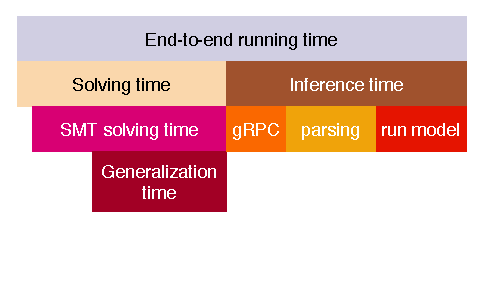
\includegraphics[width=0.6\textwidth]{figures/doping-flame.pdf}
    \caption{\mbox{Runtime~dist.~of~\dpy.}}
    \label{subfig:dpy_vs_spc_ind_gen}
	\end{subfigure}
  \centering
  \begin{subfigure}[b]{0.48\textwidth}
  \centering
    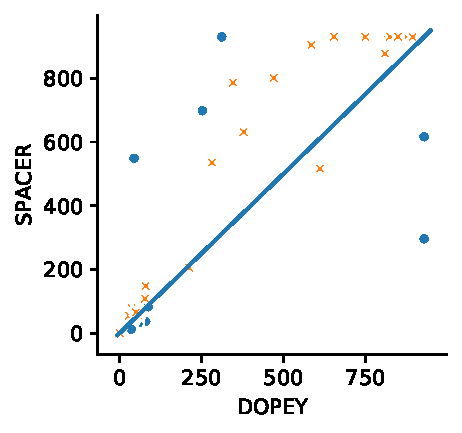
\includegraphics[width=0.99\textwidth]{figures/res-dpy_vs_spc_total.pdf}
    \caption{Solving + infer. time.}
    \label{subfig:dpy_vs_spc_total}
	\end{subfigure}
  \begin{subfigure}[b]{0.48\textwidth}
  \centering
    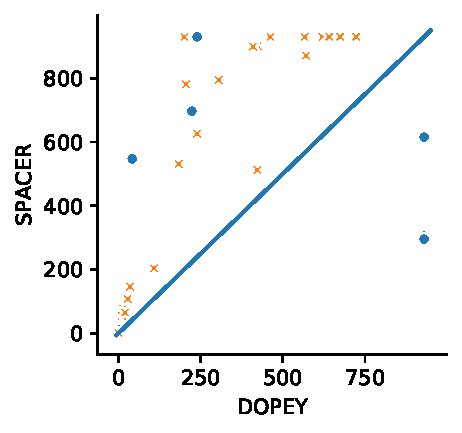
\includegraphics[width=0.99\textwidth]{figures/res-dpy_vs_spc_total_inside.pdf}
    \caption{Solving time.}
    \label{subfig:dpy_vs_spc_total_sub}
  \end{subfigure}
  \begin{subfigure}[b]{0.48\textwidth}
  \centering
    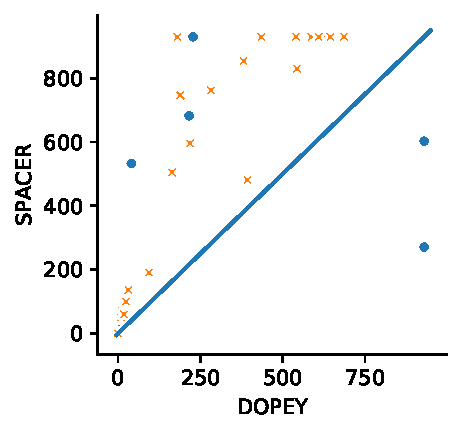
\includegraphics[width=0.99\textwidth]{figures/res-dpy_vs_spc_smt_solver.pdf}
    \caption{SMT-solving time.}
    \label{subfig:dpy_vs_spc_smt}
	\end{subfigure}
  \begin{subfigure}[b]{0.48\textwidth}
  \centering
    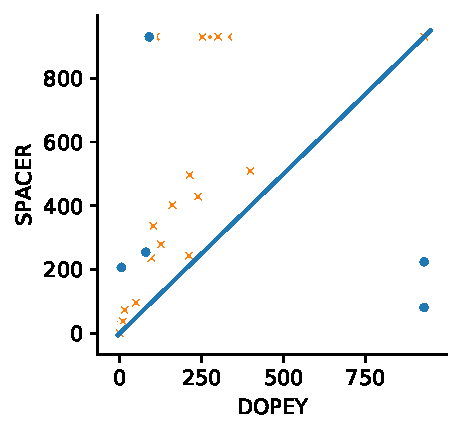
\includegraphics[width=0.99\textwidth]{figures/res-dpy_vs_spc_indgen.pdf}
    \caption{Gen. time.}
    \label{subfig:dpy_vs_spc_ind_gen_sub}
	\end{subfigure}

	\caption{Comparing \dpy's and \spc's running time, where blue dot ({\color{blue}\textbullet}) indicates an instance with unsafe property,  orange cross ({\color{orange}\textbf{x}}) indicates an instance with safe property, top (right) most place are instances \spc (\dpy) timed out.}
% 	\xs{remove the lengend, get rid of square shapes in the plot} }
  \label{fig:dpy_vs_spc}
\end{figure*}



\begin{figure}[t]
  \centering
  \begin{subfigure}{0.48\textwidth}
  \centering
    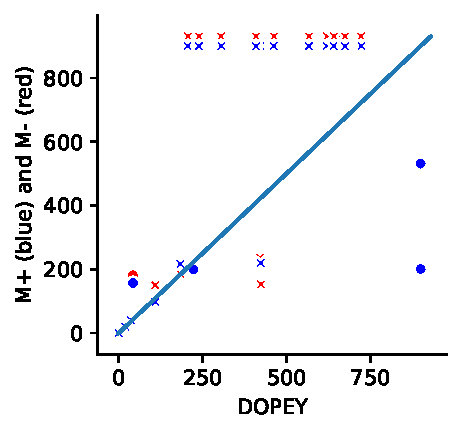
\includegraphics[width=0.99\textwidth]{figures/res-PN_vs_dpy_solving.pdf}
    \caption{Solving time.}
    \label{subfig:flame}
  \end{subfigure}
  \begin{subfigure}{0.48\textwidth}
  \centering
    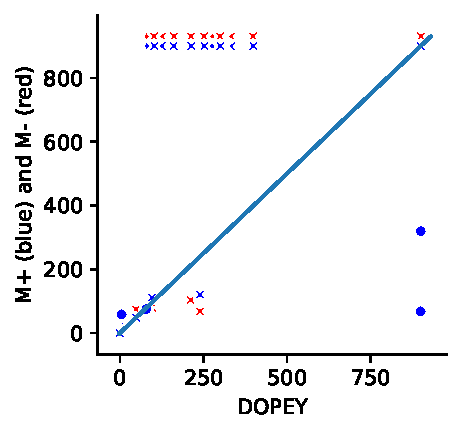
\includegraphics[width=0.99\textwidth]{figures/res-PN_vs_dpy_ind_gen.pdf}
    \caption{Gen. time.}
    \label{subfig:dpy_vs_np_total_sub}
	\end{subfigure}
\caption{\dpy vs. using only either {\color{blue}$\Mpos$} or {\color{red}$\Mneg$}.}
\label{fig:dpy_vs_np}
\end{figure}
\begin{table}[t]
  \centering
  \small
  \renewcommand{\arraystretch}{1.2}
\begin{tabular}{@{}lccc@{}}\toprule
    & All & Unsafe & Safe\\
  \midrule
    Solving + infer. time & 1.51 & 1.50 & 1.58\\
    Solving time & 2.16 & 2.46 & 2.02\\
    SMT solving time & 2.25&2.71&2.08\\
    % Generalization + infer. time & 1.58 & 1.06 &1.67\\
    Generalization time & 3.26& 3.63 & 1.67\\
    \bottomrule
\end{tabular}
\caption{\dpy's speed up compared to \spc on instances solved by both.}
\label{tab:dpy_vs_spc}
\end{table}
%%% Local Variables:
%%% mode: latex
%%% TeX-master: "0.0_main"
%%% End:


\paragraph{Implementation and optimizations.}
\tool is implemented in Python using PyTorch \cite{pytorch}, while \spc is implemented in C++. 
The communication overhead between these two could diminish the performance gain by fast inductive generation, creating an engineering challenge.  
Simply exchanging information via file IO is too expensive.
Instead, we implement a client-server architecture in which \tool is wrapped in a gRPC server connects to a gRPC client inside \spc.
As communicating and parsing over gRPC dominates the overhead, we explore further optimizations. 

% As detailed in Alg \ref{alg:qdrop}, at runtime, \spc sends over a lemma as a string, a list of literals that was kept, and , which will then be parsed in the server side using PySMT into a list of AST, then fed 

First, we use \emph{caching}. Generalizing a lemma triggers multiple requests to \tool. For each request, \dpy sends over a lemma, the server parses it and runs $\Mneg$ and $\Mpos$.
Since multiple requests over a period share the same lemma, we can parse it once and cache the result until a flag indicating \tool needs to handle a new lemma.

Second, we use \emph{parallel precomputation}. Instead of invoking $\Mneg$ and $\Mpos$ once for each literal pair, we \emph{precompute} the full co- and anti-occurrence matrices at once, and use them for \emph{all} subsequent requests.
As long as the matrices fit into the GPU memory, computing the full matrices take the same time as computing one pair of literals.

% To close the performance gap between native \spc and \dpy (\spc + gRPC + \tool), we implement multiple optimizations utilizing as much caching as possible. Recall from the discussion above that \dpy may suggests a wrong lemma candidate, so generalizing one lemma $\ell$ with \dpy may trigger more than one request to \tool. For each request, \spc has to send over a lemma, the server side has to parse it, and we need to run $\Mneg$ and $\Mpos$ to produce the candidate lemma. We want to reduce the number of parsing, and the number of time we need to call the two models.
% First, we notice that the lemma stays the same for the entire run of \tool, so we can parse it once and cache the result. This optimization also reduces the need for sending over the lemma $\ell$: we only need to send it at the beginning of the run, and only a flag indicating whether \tool has finished or not for the later requests.
% More importantly, we can \emph{precompute} the full $\Pneg$ and $\Ppos$ matrices for the lemma $\ell$, cache the results, and use them for \emph{all} the subsequent requests. Due to batching, as long as the matrices fit into the GPU memory (our GPU with 4GBs of memory can easily fit two matrices from any lemma in the benchmark during inferencing), computing the full matrices take the same time as computing one pair of literals!
Together, the two optimizations reduce overhead by up to 50\%. Although gRPC
communication and parsing still dominates the inference time, empirically it is
good enough to achieve absolute speedups. 


%%THINGS TO APE
% Combining predictions
% With our predictions of the criticality a terminalgand oftime saved by removingg, we must make a final decision onwhether or not we should removeg. To do this, we take thetop three terminals with the greatest average positive impacton synthesis time over the training set, as computed withAg. These tended to be terminals that mapped between typeswhich saved more time due to the internal mechanisms andheuristics of the CVC4 solver. We then use the final votingvector from our criticality prediction to choose only two outof the three to remove fromGto formG⋆. We chose to re-move only two terminals fromGin order to minimize thelikelihood of generating aG⋆, such thatπ(G⋆)⊆π(Gcrit).We conjecture that the number of terminals removed is agrammar-dependentparameter that must be selected on a pergrammar basis, just as the number of terminals withAg>0is grammar specific.
% Falling back to the full grammar
% There is some danger thatG⋆will, in fact, not be sufficientto synthesize a
% program. Thus, we propose a strategy that•first, tries to synthesize a program
% with the grammarG⋆•second, if synthesis withG⋆is unsuccessful, falls back
% toattempting synthesis with the full grammarG.We determine how long to wait
% before switching fromG⋆toGby finding anxthat minimizes:

%%% Local Variables:
%%% mode: latex
%%% TeX-master: "0.0_main"
%%% End:
